\documentclass[aspectratio=169,12pt]{beamer}
\usepackage{amsmath}
\usepackage{amssymb}
\usepackage{xcolor}
\usepackage[most]{tcolorbox}
\usepackage{tikz}
\usepackage{graphicx}
\usepackage[sfdefault,lf]{FiraSans}
\renewcommand{\familydefault}{\sfdefault}
\setlength{\parindent}{0pt}
\everymath{\displaystyle}
\setbeamertemplate{navigation symbols}{}
\setbeamertemplate{footline}{}
\setbeamertemplate{headline}{}
\definecolor{mmpageWhite}{HTML}{FCFBF7}
\definecolor{mmtanSoft}{HTML}{F7F5EF}
\definecolor{mmgreenDeep}{HTML}{244B2C}
\definecolor{mmgreenLeaf}{HTML}{5D8A56}
\definecolor{mmtext}{HTML}{163221}
\definecolor{mmanswerColor}{HTML}{306A3A}
\setbeamercolor{background canvas}{bg=mmpageWhite}
\setbeamercolor{normal text}{fg=mmtext,bg=mmpageWhite}
\newtcolorbox{MMCard}[1][]{enhanced,breakable=false,colback=white,colframe=black,boxrule=1.5pt,arc=8pt,left=4pt,right=4pt,top=4pt,bottom=4pt,before skip=0pt,after skip=0pt,height=0.40\textheight,valign=center,#1}
\newcommand{\KoruIcon}{\raisebox{-0.2em}{
\includegraphics[height=1.05em]{img/header-logo.png}}}
\newcommand{\HoeIcon}{\raisebox{-0.2em}{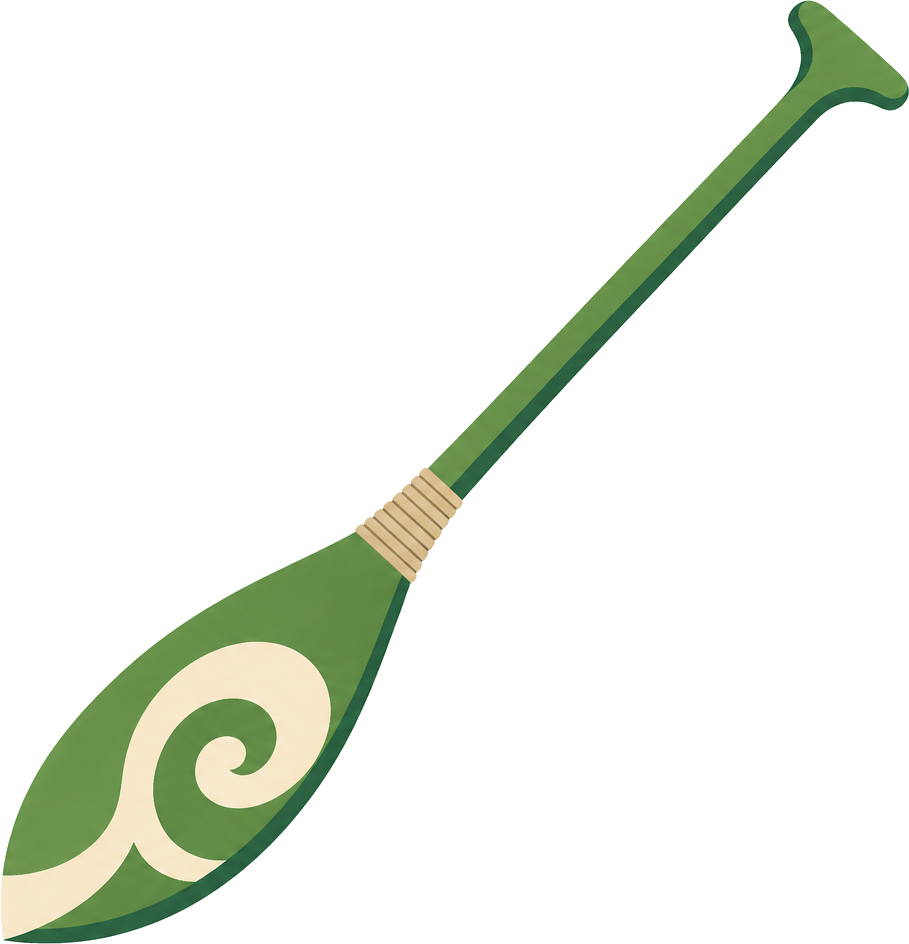
\includegraphics[height=1.05em]{img/hoe.png}}}
\newcommand{\ScaffoldIcons}[1]{\ifcase#1\or \HoeIcon\or \HoeIcon\hspace{0.22em}\HoeIcon\or \HoeIcon\hspace{0.22em}\HoeIcon\hspace{0.22em}\HoeIcon\fi}
\newcommand{\WorksheetTitle}[2]{%
  {\colorbox{mmtanSoft}{\parbox[c][2.2em][c]{0.975\linewidth}{%
    \hspace{0.25em}{\Large\bfseries\textcolor{mmgreenDeep}{#1}\hfill\ScaffoldIcons{#2}}}}
  \par\vspace{0.12em}{\color{mmgreenLeaf}\rule{\linewidth}{2.5pt}}\par\vspace{0.06em}}
}
\newcommand{\BigSym}[1]{\begin{center}\scalebox{0.7}{#1}\end{center}}
\newcommand{\SymQ}[2]{\begin{MMCard}\centering\vfill\BigSym{#1}\vspace{0.1em}{\raggedright\small\textbf{#2}}\vfill\end{MMCard}}
\newcommand{\SymAns}[3]{\begin{MMCard}\centering\vfill\BigSym{#1}\vspace{0.08em}{\raggedright\small\textbf{#2}\par\textcolor{mmanswerColor}{\bfseries #3}}\vfill\end{MMCard}}
\setbeamertemplate{background}{
 \begin{tikzpicture}[remember picture,overlay]
 \draw[black,line width=1.5pt,rounded corners=10pt]
 ([xshift=0.45cm,yshift=-0.45cm]current page.north west)
 rectangle
 ([xshift=-0.45cm,yshift=0.45cm]current page.south east);
 \end{tikzpicture}
}
\begin{document}

\begin{frame}[t]
\WorksheetTitle{Start Tasks - Nets}{1}
\vspace{-0.1em}
\begin{columns}[T,onlytextwidth]
\begin{column}{0.33\textwidth}
\SymAns{\tikz{\draw[thick] (0,0) rectangle (1,1); \draw[thick] (0,-1) rectangle (1,0); \draw[thick] (0,-2) rectangle (1,-1); \draw[thick] (1,-1) rectangle (2,0); \draw[thick] (-1,-1) rectangle (0,0); \draw[thick] (2,-1) rectangle (3,0); \node[scale=0.5] at (0.5,-0.5) {1}; \node[scale=0.5] at (0.5,-1.5) {2}; \node[scale=0.5] at (1.5,-0.5) {3}; \node[scale=0.5] at (-0.5,-0.5) {4}; \node[scale=0.5] at (2.5,-0.5) {5}; \node[scale=0.5] at (0.5,0.5) {6};}}{1. Faces in this net?}{6}
\SymAns{\tikz{\draw[thick] (0,0) rectangle (1,1); \draw[thick] (0,-1) rectangle (1,0); \draw[thick] (0,-2) rectangle (1,-1); \draw[thick] (1,-1) rectangle (2,0); \draw[thick] (-1,-1) rectangle (0,0); \draw[thick] (2,-1) rectangle (3,0); \node[scale=0.5] at (0.5,-0.5) {1}; \node[scale=0.5] at (0.5,-1.5) {2}; \node[scale=0.5] at (1.5,-0.5) {3}; \node[scale=0.5] at (-0.5,-0.5) {4}; \node[scale=0.5] at (2.5,-0.5) {5}; \node[scale=0.5] at (0.5,0.5) {6};}}{2. Faces should a cube net have?}{6}
\end{column}

\begin{column}{0.33\textwidth}
\SymAns{\tikz{\draw[thick] (0,0) rectangle (1,1); \draw[thick] (0,-1) rectangle (1,0); \draw[thick] (0,-2) rectangle (1,-1); \draw[thick] (1,-1) rectangle (2,0); \draw[thick] (-1,-1) rectangle (0,0); \draw[thick] (2,-1) rectangle (3,0); \node[scale=0.5] at (0.5,-0.5) {1}; \node[scale=0.5] at (0.5,-1.5) {2}; \node[scale=0.5] at (1.5,-0.5) {3}; \node[scale=0.5] at (-0.5,-0.5) {4}; \node[scale=0.5] at (2.5,-0.5) {5}; \node[scale=0.5] at (0.5,0.5) {6};}}{3. Opposite the bottom face?}{The top face (face 6)}
\SymAns{\tikz{\draw[thick] (0,0) rectangle (1,1); \draw[thick] (0,-1) rectangle (1,0); \draw[thick] (0,-2) rectangle (1,-1); \draw[thick] (1,0) rectangle (2,1); \draw[thick] (1,1) rectangle (2,2); \draw[thick] (-1,0) rectangle (0,1);}}{4. Does T-shape form a cube?}{Yes — it is a valid cube net}
\end{column}

\begin{column}{0.33\textwidth}
\SymAns{\tikz{\draw[thick] (0,0) rectangle (1,1); \draw[thick] (0,-1) rectangle (1,0); \draw[thick] (0,-2) rectangle (1,-1); \draw[thick] (1,0) rectangle (2,1); \draw[thick] (1,1) rectangle (2,2); \draw[thick] (-1,0) rectangle (0,1);}}{5. Faces of a cube?}{6}
\SymAns{\tikz{\draw[thick] (0,0) rectangle (2,1); \draw[thick] (0,-1) rectangle (2,0); \draw[thick] (0,-2) rectangle (2,-1); \draw[thick] (2,-1) rectangle (3,0); \draw[thick] (-1,-1) rectangle (0,0); \draw[thick] (0,1) rectangle (2,2); \node[scale=0.4] at (1,0.5) {5}; \node[scale=0.4] at (1,-1.5) {2}; \node[scale=0.4] at (1,-0.5) {3}; \node[scale=0.4] at (-0.5,-0.5) {4}; \node[scale=0.4] at (2.5,-0.5) {5};}}{6. Faces of a cuboid?}{6}
\end{column}
\end{columns}
\end{frame}

\begin{frame}[t]
\WorksheetTitle{Start Tasks - Nets}{1}
\vspace{-0.1em}
\begin{columns}[T,onlytextwidth]
\begin{column}{0.33\textwidth}
\SymAns{\tikz{\draw[thick] (0,0) rectangle (2,1); \draw[thick] (0,-1) rectangle (2,0); \draw[thick] (0,-2) rectangle (2,-1); \draw[thick] (2,-1) rectangle (3,0); \draw[thick] (-1,-1) rectangle (0,0); \draw[thick] (0,1) rectangle (2,2); \node[scale=0.4] at (1,0.5) {5}; \node[scale=0.4] at (1,-1.5) {2}; \node[scale=0.4] at (1,-0.5) {3}; \node[scale=0.4] at (-0.5,-0.5) {4}; \node[scale=0.4] at (2.5,-0.5) {5};}}{7. What 3D shape?}{Cuboid (rectangular prism)}
\SymAns{\tikz{\draw[thick] (0,0) rectangle (1,1); \draw[thick] (1,0) rectangle (2,1); \draw[thick] (2,0) rectangle (3,1); \draw[thick] (0,-1) rectangle (1,0); \draw[thick] (0,1) rectangle (1,2);}}{8. Missing what?}{The lid / top face}
\end{column}

\begin{column}{0.33\textwidth}
\SymAns{\tikz{\draw[thick] (0,0) rectangle (1,1); \draw[thick] (1,0) rectangle (2,1); \draw[thick] (2,0) rectangle (3,1); \draw[thick] (0,-1) rectangle (1,0); \draw[thick] (0,1) rectangle (1,2);}}{9. Faces when folded?}{5 (open box, no lid)}
\SymAns{\tikz{\draw[thick] (0,0)--(1,0)--(1.5,-0.866)--(0.5,-0.866)--cycle; \draw[thick] (0,0)--(-0.5,0.866)--(0.5,0.866)--(1,0); \draw[thick] (-0.5,0.866)--(-1.5,0)--(-0.5,-0.866)--(0.5,-0.866);}}{10. Pyramid faces?}{5 (1 square + 4 triangles)}
\end{column}

\begin{column}{0.33\textwidth}
\SymAns{\tikz{\draw[thick] (0,0)--(1,0)--(1.5,-0.866)--(0.5,-0.866)--cycle; \draw[thick] (0,0)--(-0.5,0.866)--(0.5,0.866)--(1,0); \draw[thick] (-0.5,0.866)--(-1.5,0)--(-0.5,-0.866)--(0.5,-0.866);}}{11. Triangular faces meet at?}{The apex (vertex at top)}
\SymAns{\tikz{\draw[thick] (0,0)--(1,0)--(0.5,-0.866)--cycle; \draw[thick] (1,0)--(2,0)--(2,1)--(1,1)--cycle; \draw[thick] (0,0)--(0,1)--(1,1)--(1,0); \draw[thick] (0,1)--(0.5,0.134); \draw[thick] (1,1)--(2,1)--(2.5,0.134)--(0.5,0.134);}}{12. Triangular prism faces?}{5}
\end{column}
\end{columns}
\end{frame}

\begin{frame}[t]
\WorksheetTitle{Start Tasks - Nets}{1}
\vspace{-0.1em}
\begin{columns}[T,onlytextwidth]
\begin{column}{0.33\textwidth}
\SymAns{\tikz{\draw[thick] (0,0)--(1,0)--(0.5,-0.866)--cycle; \draw[thick] (1,0)--(2,0)--(2,1)--(1,1)--cycle; \draw[thick] (0,0)--(0,1)--(1,1)--(1,0); \draw[thick] (0,1)--(0.5,0.134); \draw[thick] (1,1)--(2,1)--(2.5,0.134)--(0.5,0.134);}}{13. Rectangular faces?}{3}
\SymAns{\tikz{\draw[thick] (0,0) rectangle (2,1); \draw[thick] (0,-1) rectangle (2,0); \draw[thick] (0,-2) rectangle (2,-1); \draw[thick] (0,1) rectangle (2,2); \draw[thick] (0,2) rectangle (2,3); \draw[thick] (2,0)--(2.5,0.866)--(2.5,1.866)--(2,2.732)--(0,2.732);}}{14. Hexagonal prism faces?}{8 (6 rectangular + 2 hexagonal)}
\end{column}

\begin{column}{0.33\textwidth}
\SymAns{\tikz{\draw[thick] (0,0) rectangle (2,1); \draw[thick] (0,-1) rectangle (2,0); \draw[thick] (0,-2) rectangle (2,-1); \draw[thick] (0,1) rectangle (2,2); \draw[thick] (0,2) rectangle (2,3); \draw[thick] (2,0)--(2.5,0.866)--(2.5,1.866)--(2,2.732)--(0,2.732);}}{15. Rectangular faces?}{4 visible in this net}
\SymAns{\tikz{\draw[thick] (0,0) rectangle (1,1); \draw[thick] (0,-1) rectangle (1,0); \draw[thick] (0,-2) rectangle (1,-1); \draw[thick] (1,-1) rectangle (2,0); \draw[thick] (-1,-1) rectangle (0,0); \draw[thick] (2,-1) rectangle (3,0); \node[scale=0.5] at (0.5,-0.5) {1}; \node[scale=0.5] at (0.5,-1.5) {2}; \node[scale=0.5] at (1.5,-0.5) {3}; \node[scale=0.5] at (-0.5,-0.5) {4}; \node[scale=0.5] at (2.5,-0.5) {5}; \node[scale=0.5] at (0.5,0.5) {6};}}{16. Distinct cube nets?}{11}
\end{column}

\begin{column}{0.33\textwidth}
\SymAns{\tikz{\draw[thick] (0,0) rectangle (1,1); \draw[thick] (0,-1) rectangle (1,0); \draw[thick] (0,-2) rectangle (1,-1); \draw[thick] (1,-1) rectangle (2,0); \draw[thick] (-1,-1) rectangle (0,0); \draw[thick] (2,-1) rectangle (3,0); \node[scale=0.5] at (0.5,-0.5) {1}; \node[scale=0.5] at (0.5,-1.5) {2}; \node[scale=0.5] at (1.5,-0.5) {3}; \node[scale=0.5] at (-0.5,-0.5) {4}; \node[scale=0.5] at (2.5,-0.5) {5}; \node[scale=0.5] at (0.5,0.5) {6};}}{17. Shape of each cube face?}{Square}
\SymAns{\tikz{\draw[thick] (0,0) rectangle (1,1); \draw[thick] (0,-1) rectangle (1,0); \draw[thick] (0,-2) rectangle (1,-1); \draw[thick] (1,-2) rectangle (2,-1); \draw[thick] (-1,-2) rectangle (0,-1);}}{18. Open box from pentomino A?}{Check by folding mentally}
\end{column}
\end{columns}
\end{frame}

\begin{frame}[t]
\WorksheetTitle{Start Tasks - Nets}{1}
\vspace{-0.1em}
\begin{columns}[T,onlytextwidth]
\begin{column}{0.33\textwidth}
\SymAns{\tikz{\draw[thick] (0,0) rectangle (1,1); \draw[thick] (1,0) rectangle (2,1); \draw[thick] (0,-1) rectangle (1,0); \draw[thick] (0,-2) rectangle (1,-1); \draw[thick] (1,-2) rectangle (2,-1);}}{19. Open box from pentomino B?}{Check by folding mentally}
\SymAns{\tikz{\draw[thick] (0,0)--(1,0)--(0.5,-0.866)--cycle; \draw[thick] (0,0)--(-0.5,0.866)--(0.5,0.866)--(1,0); \draw[thick] (0.5,-0.866)--(1.5,-0.866)--(1,0);}}{20. Tetrahedron faces?}{4}
\end{column}

\begin{column}{0.33\textwidth}
\SymAns{\tikz{\draw[thick] (0,0)--(1,0)--(0.5,-0.866)--cycle; \draw[thick] (0,0)--(-0.5,0.866)--(0.5,0.866)--(1,0); \draw[thick] (0.5,-0.866)--(1.5,-0.866)--(1,0);}}{21. Faces shape?}{Triangle (equilateral)}
\SymAns{\tikz{\draw[thick] (0,0) rectangle (1,1); \draw[thick] (0,-1) rectangle (1,0); \draw[thick] (0,-2) rectangle (1,-1); \draw[thick] (1,-1) rectangle (2,0); \draw[thick] (-1,-1) rectangle (0,0); \draw[thick] (2,-1) rectangle (3,0); \foreach \x in {0,2} \foreach \y in {0,2} \fill[black] (\x*0.5+0.25,\y*0.5-1.5+0.25) circle (0.06); \fill[black] (0.25,-0.75) circle (0.06);}}{22. Opposite faces sum?}{7}
\end{column}

\begin{column}{0.33\textwidth}
\SymAns{\tikz{\draw[thick] (0,0) rectangle (1,1); \draw[thick] (0,-1) rectangle (1,0); \draw[thick] (0,-2) rectangle (1,-1); \draw[thick] (1,-1) rectangle (2,0); \draw[thick] (-1,-1) rectangle (0,0); \draw[thick] (2,-1) rectangle (3,0); \foreach \x in {0,2} \foreach \y in {0,2} \fill[black] (\x*0.5+0.25,\y*0.5-1.5+0.25) circle (0.06); \fill[black] (0.25,-0.75) circle (0.06);}}{23. Opposite faces sum to?}{7 on a standard die}
\SymAns{\tikz{\draw[thick] (0,0) rectangle (3,1); \draw[thick] (0,-1) rectangle (3,0); \draw[thick] (1.5,0)--(1.5,1); \draw[thick] (0,1)--(0,1.5)--(1.5,2)--(3,1.5)--(3,1); \node[scale=0.4] at (1.5,-0.5) {3 m}; \node[scale=0.4] at (1.5,1.5) {2 m};}}{24. Triangular faces?}{2}
\end{column}
\end{columns}
\end{frame}

\begin{frame}[t]
\WorksheetTitle{Start Tasks - Nets}{1}
\vspace{-0.1em}
\begin{columns}[T,onlytextwidth]
\begin{column}{0.33\textwidth}
\SymAns{\tikz{\draw[thick] (0,0) rectangle (3,1); \draw[thick] (0,-1) rectangle (3,0); \draw[thick] (1.5,0)--(1.5,1); \draw[thick] (0,1)--(0,1.5)--(1.5,2)--(3,1.5)--(3,1); \node[scale=0.4] at (1.5,-0.5) {3 m}; \node[scale=0.4] at (1.5,1.5) {2 m};}}{25. Total faces on tent?}{5 (2 triangles + 3 rectangles)}
\SymAns{\tikz{\draw[thick] (0,0) rectangle (1,1); \draw[thick] (1,0) rectangle (2,1); \draw[thick] (2,0) rectangle (3,1); \draw[thick] (2,1) rectangle (3,2); \draw[thick] (2,2) rectangle (3,3);}}{26. Open box from L-shape?}{Check by folding mentally}
\end{column}

\begin{column}{0.33\textwidth}
\SymAns{\tikz{\draw[thick] (0,0) rectangle (1,1); \draw[thick] (0,-1) rectangle (1,0); \draw[thick] (0,-2) rectangle (1,-1); \draw[thick] (1,-1) rectangle (2,0); \draw[thick] (-1,-1) rectangle (0,0); \draw[thick] (2,-1) rectangle (3,0); \node[scale=0.5] at (0.5,-0.5) {1}; \node[scale=0.5] at (0.5,-1.5) {2}; \node[scale=0.5] at (1.5,-0.5) {3}; \node[scale=0.5] at (-0.5,-0.5) {4}; \node[scale=0.5] at (2.5,-0.5) {5}; \node[scale=0.5] at (0.5,0.5) {6};}}{27. 3D shape name?}{Cube}
\end{column}

\begin{column}{0.33\textwidth}
\end{column}
\end{columns}
\end{frame}
\end{document}